\documentclass{article}
\usepackage{graphicx}
\usepackage{amsmath}
\usepackage{cite}
\usepackage{color}
\usepackage{enumitem}
\usepackage{natbib}
\usepackage{tabularx}
\usepackage{natbib}
\usepackage{ragged2e}
\usepackage{geometry}
\geometry{a4paper, left=3.5 cm, right=3.5 cm, top=3 cm, bottom=3 cm}

\title{\huge\textbf{La digitalizzazione nelle PA}}
\author{\texttt{Alessandro Meloni 0001118676 GEPID}}
\date{Anno accademico 2023/2024}

\renewcommand\contentsname{Indice}
\renewcommand\refname{Bibliografia}

\begin{document}
\begin{figure}
    \centering
    
\includegraphics[width=0.9\linewidth]{Uniboarms.png}
\end{figure}
\maketitle

\centering \tableofcontents

\newpage\centering
\section{Introduzione}
\begin{justify}
L'ampliamento di tecnologie che usufruiscono di intelligenza artificiale è un fatto che agli occhi di tutti è percepito in questo preciso momento storico. L'errore che si fa però è pensare che l'AI sia un fatto recente, in realtà i primi studi pubblicati sulle reti neurali risalgono al 1943, pertanto gli studi informatici a riguardo hanno circa 50 anni.\citep{mcculloch1943logical}\\ Usufruiscono di sistemi di intelligenza artificale anche il riconoscimento delle spam nella posta elettronica (anni 90); oppure ancora il riconoscimento della scrittura. Semplicemente ora siamo in un momento storico dove si è compresa l'enorme potenzialità di questi algoritmi, la loro capacità di poter "ingerire" informazioni e processarle in modo ottimale.\\
L'Italia in termini di investimenti risulta essere un po' indietro rispetto ad altre realtà europee, però parallelamente si sta facendo un grosso passa avanti nel cercare di far combaciare l'algoretica con bisogni economici digitali (per \textit{algoretica} si intende riuscire a far combaciare l'utilizzo degli algoritmi e dell'etica in modo tale che non si vadano a creare delle soluzioni disumanizzate).
Di fatto lo sviluppo delle tecnologie odierne, sappiamo tutti, sta aprendo un forte dibattito, pertanto, risulta opportuno avere una corretta regolamentazione sia a livello statale che sovrastatale.
In Italia ci sono varie aurorità che si occupano del settore della digitalizzazione, ognuno con particolari compiti.
Sono tutti degli enti molto complessi che tentano di accompagnare l'Italia verso un completa transizione digitale, dati dall'avvento di numerose tecnologie quali Blockchain, Ai e via discorrendo.\\
Nello specifico si analizzeranno gli articoli che sanciscono i principi digitali del nuovo codice dei contratti pubblici: d.lgs 36/2023, ma prevalente nell'art 30: utilizzo di meccanismi automatizzati nel ciclo di vita dei contratti pubblici. Ragion per cui bisognerà preventivamente comprendere i principi cardine enunciati dagli artt 19 a 29.\\
Trasversalmente verranno anche spiegate le funzioni dell'ANAC e la regolamentazione delle Autorità Amministrative Indipendenti, ma senza allontarsi troppo dal topic centrale, così da dare una visione di insieme più corretta e comprensibile.\\
Infine si vedranno a che punto è la regolamentazione UE sull'AI e gli obiettivi che specialmente in Italia si hanno tramite l'ausilio dei fondi del PNRR.
Con questo paper si cerca di analizzare oggettivamente quali potrebbero essere le ripercussioni a livello organizzativo, nel mondo del lavoro e anche nel rispetto dei principi amministrativi dedotti dall'art 97 della Costituzione, senza dimenticarsi dei collegamenti con le varie leggi specifiche in materia.
\end{justify}

\centering
\section{Nuovo codice degli appalti}
\begin{justify}
    
\end{justify}

\newpage\subsection{Digitalizzazione dei contratti e principi}
\begin{justify}
    Esempio.
\end{justify}

\subsection{Art 30 d.lgs 36/2023}
\begin{justify}
    Esempio.
\end{justify}


\subsection{AI ACT e PNRR}
\begin{center}
    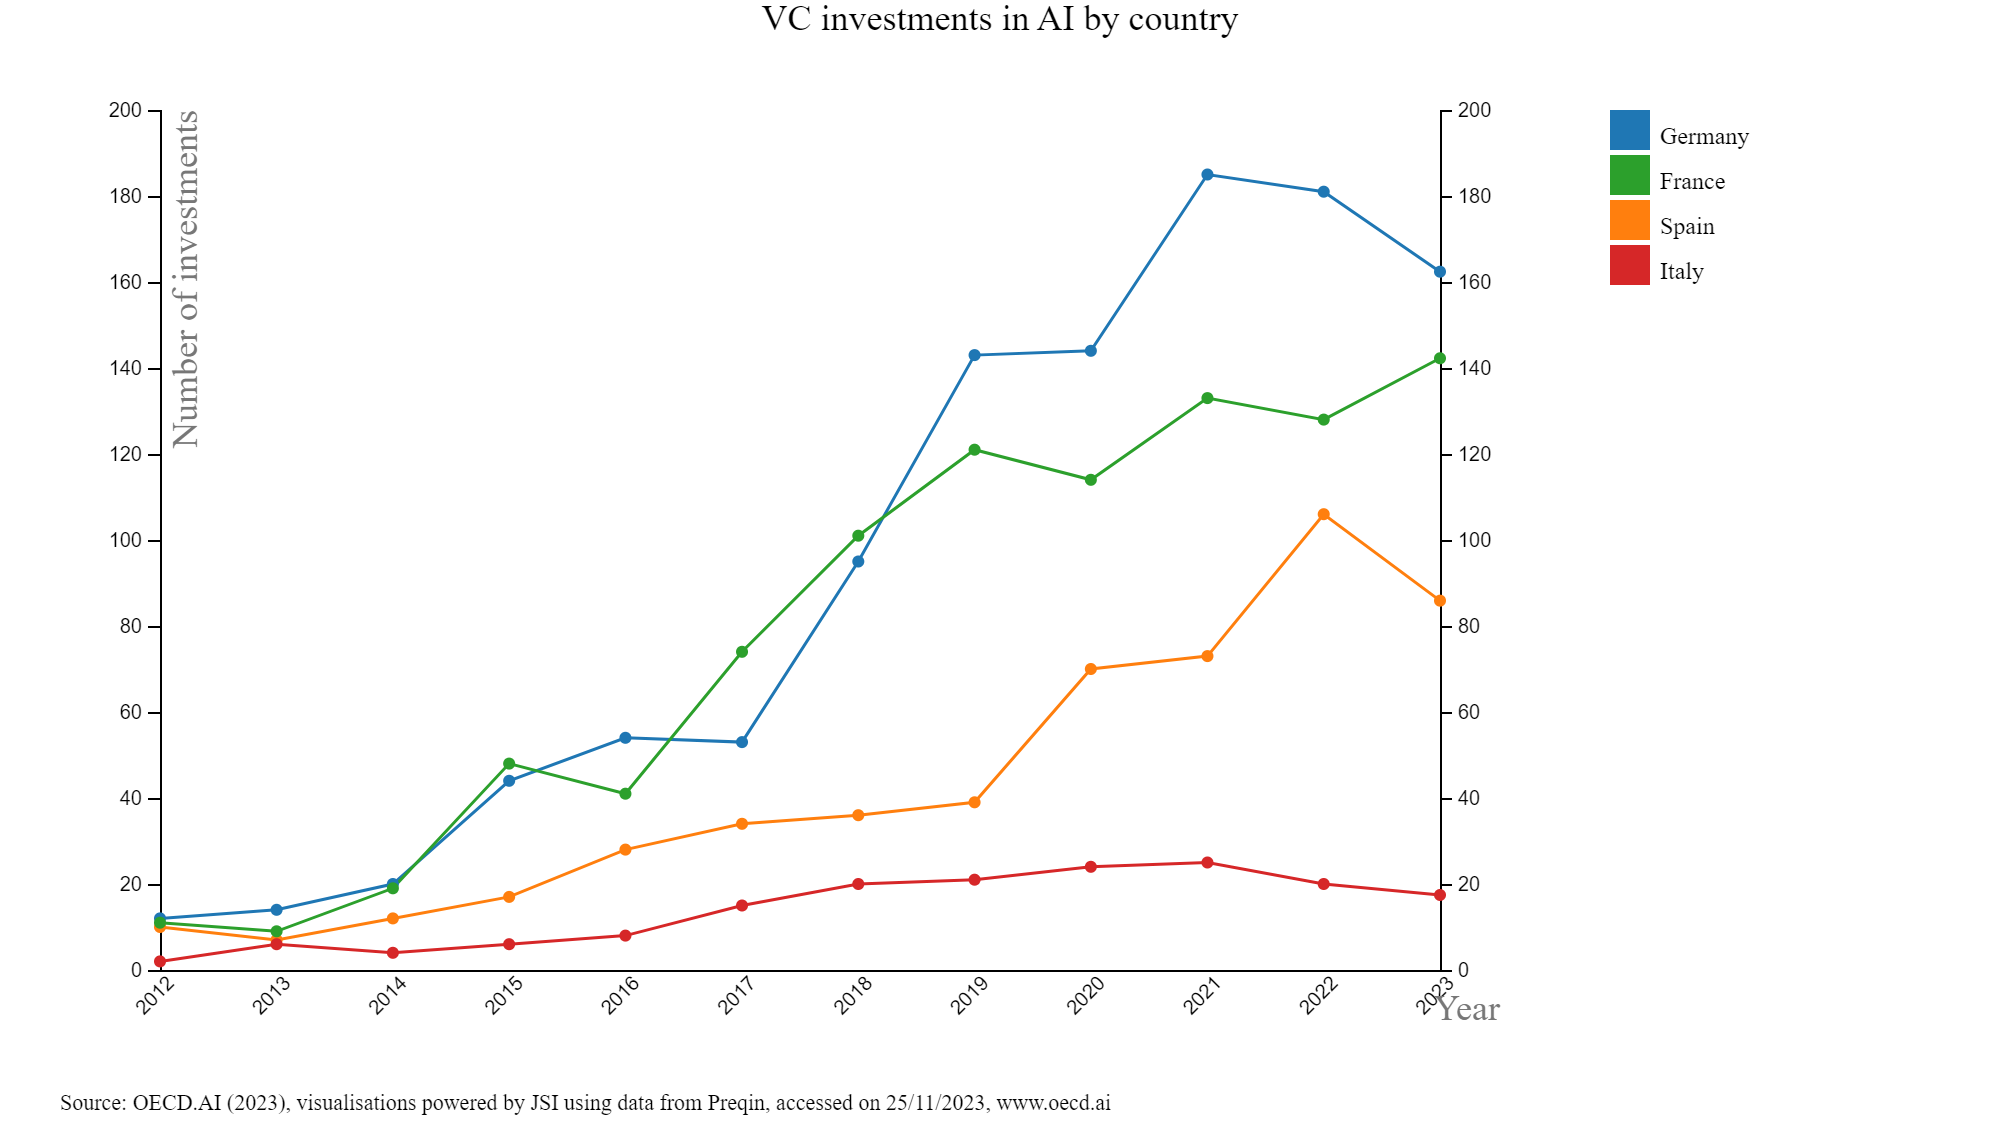
\includegraphics[width=0.3\linewidth]{Numero investimenti.png}
\end{center}
\begin{justify}
    Questo grafico rappresenta il numero degli investimenti effettuati per Stato nel settore AI e Data.
\end{justify}

\begin{center}
    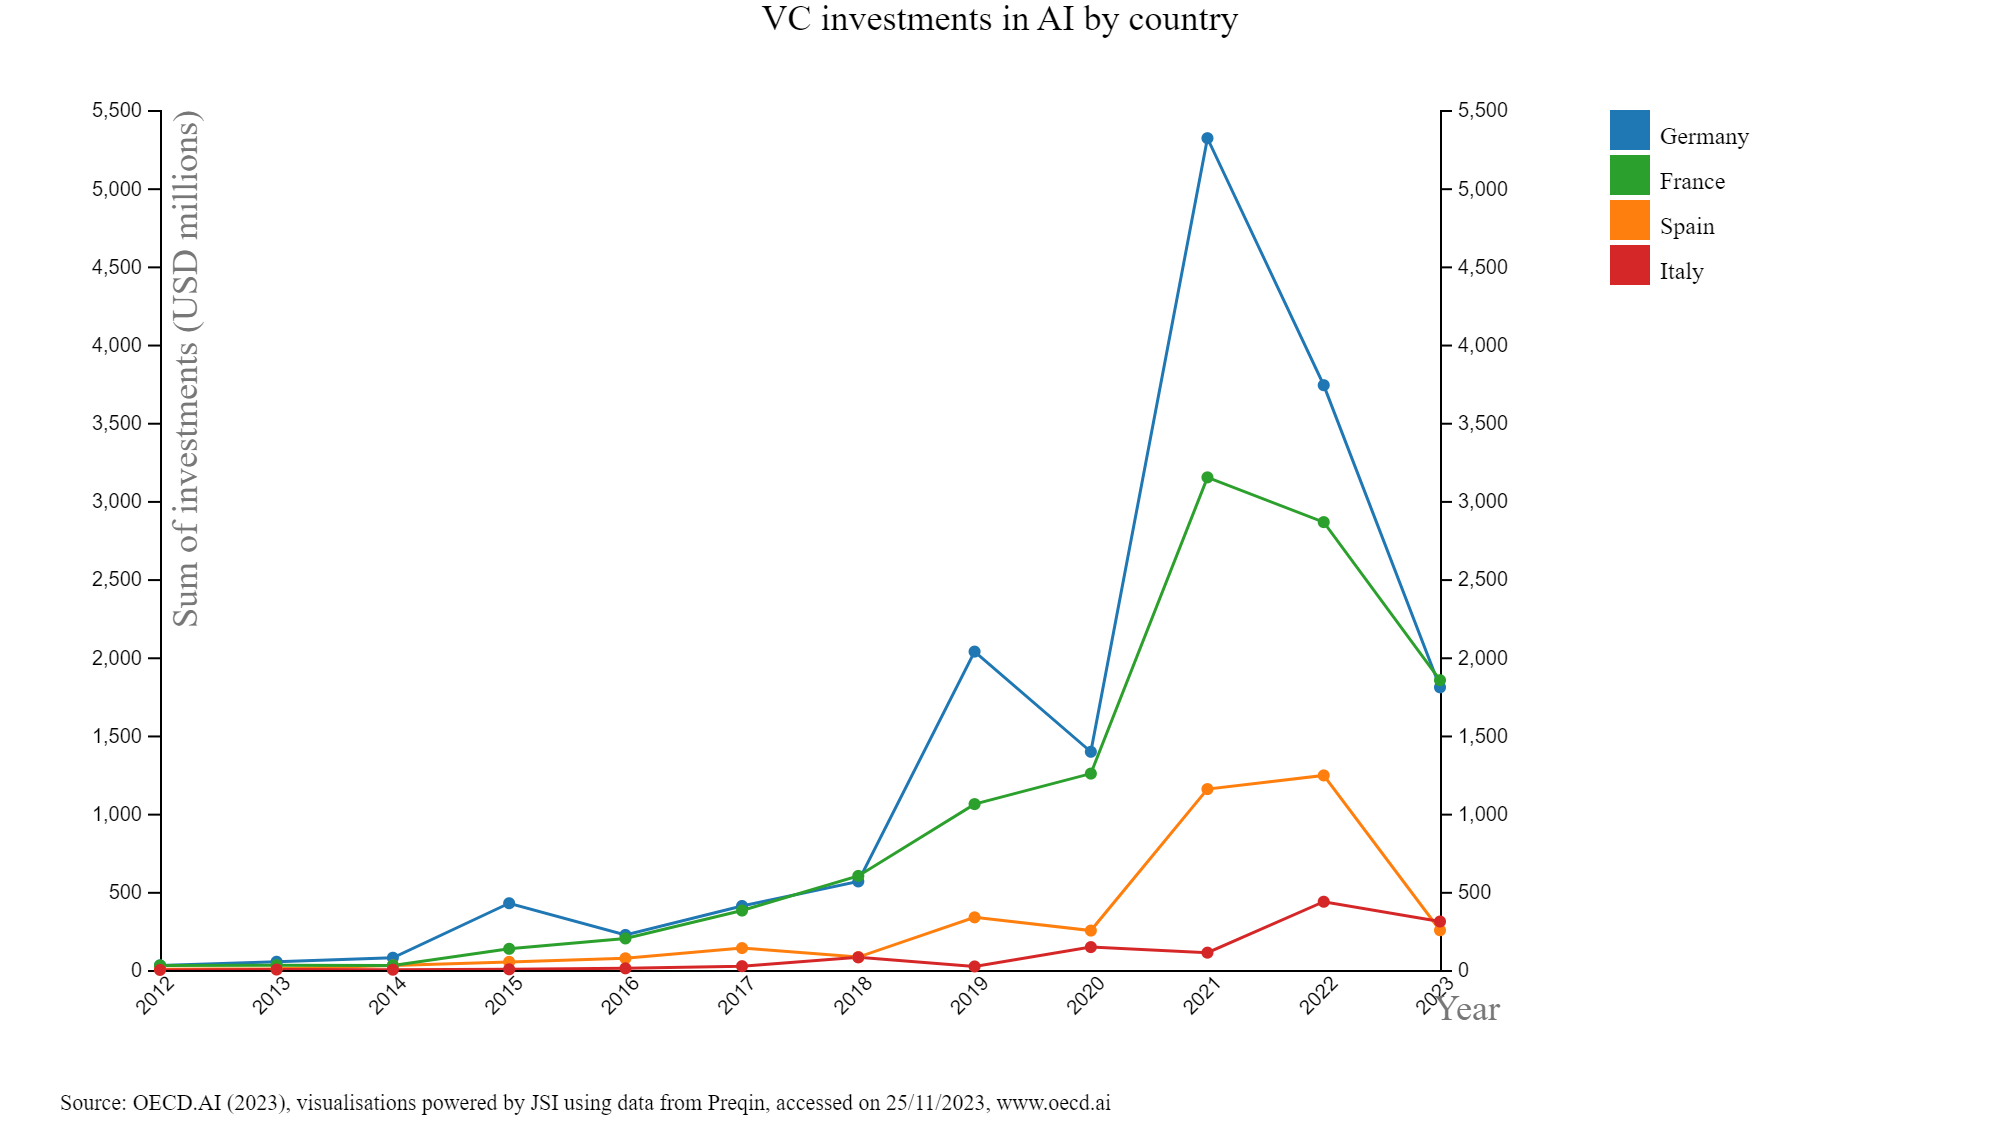
\includegraphics[width=0.3\linewidth]{Somma degli investimenti.png}
\end{center}
\begin{justify}
    Questo invece lo rappresenta sulla base dei milioni di dollari spesi in questo settore.
\end{justify}

\newpage \centering
\section{Conclusione e opinioni finali}
\begin{justify}
    L'ANAC è un ente alla quale mi sono avvicinato durante il periodo di studio triennale, tramite un tirocinio svoltosi presso l'Ufficio Anticorruzione del Comune di Cagliari. 
\end{justify}

\begin{justify}
    \bibliography{Bibliografia}
    \bibliographystyle{plainnat}
\end{justify}
\end{document}